\chapter{Locality of constraints}\label{ch:locality}

Is the topology of the history space a consequence of integer divisibility, or of the \emph{form} of the constraint? This chapter answers for one precisely stated class. A \emph{pairwise grammar} specifies, for every ordered pair of labels, whether the first may be immediately followed by the second; histories are the orderings all of whose consecutive pairs are allowed. No integers, no divisibility. For six labels we prove that such a grammar never produces a two-dimensional hole. Constraints on consecutive \emph{triples} can, and so can prefix-set constraints. The dividing line is how local the forbidden pattern is. Every statement here is for six labels; no version for other lengths is claimed.

\section{Adjacency complexes}\label{sec:adjacency}
Let $G$ be a digraph on $[6]$ and $A_G$ the set of orderings $(x_1,\dots,x_6)$ with $(x_t,x_{t+1})\in G$ for all $t$. Such $A_G$ is not prefix-defined in general. Let $B$ be the set of ordered pairs $p=(x,y)$, $x\ne y$, not in $G$; an ordering is non-admissible iff $x$ is immediately followed by $y$ for some $p\in B$. For $p=(x,y)$ let $Z_p\subseteq T$ be the subcomplex generated by the flags in which $x$ is immediately followed by $y$, and $Z_S=\bigcap_{p\in S}Z_p$. Then
\[
Y_{A_G}=\bigcup_{p\in B}Z_p .
\]
\begin{lemma}[description of $Z_S$; analytic]\label[lemma]{lem:Z}
A simplex of $T$, written as an ordered partition $(B_1|\dots|B_m)$ with block index $b:[6]\to\{1,\dots,m\}$, $m\ge2$, lies in $Z_{(x,y)}$ iff $b(y)-b(x)\in\{0,1\}$. Hence $Z_S$ consists of the ordered partitions with $b(y)-b(x)\in\{0,1\}$ for all $(x,y)\in S$. Moreover $Z_S\neq\emptyset$ iff the digraph $([6],S)$ is not strongly connected; in particular $Z_S\ne\emptyset$ whenever $|S|\le5$.

\end{lemma}
\begin{proof}
A flag refining the partition has $x$ immediately before $y$ iff either $x,y$ lie in the same block (they can be listed consecutively in that order) or $x$ is last in $B_i$ and $y$ first in $B_{i+1}$; conversely adjacency forces $b(y)-b(x)\in\{0,1\}$. Intersections follow. For non-emptiness: $Z_S$ is closed under coarsening (merging adjacent blocks keeps $b(y)-b(x)\in\{0,1\}$), so it is nonempty iff it has a vertex, i.e.\ a $2$-block partition $(I|I^c)$ with $b(y)-b(x)\in\{0,1\}$ for $(x,y)\in S$; this fails exactly when $y\in I$, $x\notin I$, so such $I$ is a proper nonempty set closed under in-neighbours of $S$. A proper nonempty in-closed set exists iff the digraph is not strongly connected (in a strongly connected digraph an in-closed nonempty set is everything; otherwise a source strong component is in-closed and proper). A strongly connected digraph on $6$ vertices has at least $6$ arcs, so $|S|\le5$ forces non-strong-connectivity.
\end{proof}

\section{The pairwise-adjacency theorem}
\begin{theorem}[locality theorem for pairwise grammars; computer-assisted]\label[theorem]{thm:pairwise}
Let $k=6$, let $G$ be any digraph on six distinguishable events and $\emptyset\neq A_G\subsetneq S_6$. Then $\beta_2(K_{A_G};\F)=0$. In particular this holds for every symbolic grammar over a finite alphabet in which admissibility is a conjunction of constraints on consecutive pairs of categories, with arbitrary category multisets.

\end{theorem}
The proof reduces the statement to three finite facts about the thirty ordered pairs.
\begin{enumerate}[label=(F\arabic*)]
\item for each of the $30$ ordered pairs $p$: $Z_p$ is nonempty and $\Hh_0(Z_p)=\Hh_1(Z_p)=0$;
\item for each of the $\binom{30}{2}=435$ sets $\{p,q\}$: $Z_{pq}$ is nonempty and connected;
\item for each of the $\binom{30}{3}=4060$ sets $\{p,q,r\}$: $Z_{pqr}$ is nonempty.
\end{enumerate}
\begin{proof}[Proof of \cref{thm:pairwise} from (F1)--(F3)]
Let $B\neq\emptyset$ be the set of bad pairs. Consider the double complex $C_{a,q}=\bigoplus_{S\subseteq B,\,|S|=a+1}C_q(Z_S;\F)$ with horizontal differential the sum (over $\F$ signs are irrelevant) of the maps induced by the inclusions $Z_S\hookrightarrow Z_{S\setminus\{p\}}$ and vertical differential the simplicial boundary, augmented by $C_{0,q}\to C_q(Y)$. For a fixed simplex $\sigma$ of $Y$, its contribution to the horizontal direction is the augmented chain complex of the full simplex on $B_\sigma=\{p\in B:\ \sigma\in Z_p\}\neq\emptyset$, which is exact. Hence the total homology is $H_*(Y_{A_G})$, and filtering the other way gives the Mayer--Vietoris (\v Cech) spectral sequence $E^1_{a,q}=\bigoplus_{|S|=a+1}H_q(Z_S)\Rightarrow H_{a+q}(Y_{A_G})$.
Total degree $1$ involves only $E_{0,1}$ and $E_{1,0}$. By (F1), $E^1_{0,1}=\bigoplus_pH_1(Z_p)=0$. For $E_{1,0}$: by (F1)--(F3), $E^1_{0,0}=\F^B$, $E^1_{1,0}=\F^{\binom B2}$ (all $Z_{pq}$ connected), and $E^1_{2,0}=\bigoplus_{\{p,q,r\}}H_0(Z_{pqr})$ with each summand a nonzero space whose basis elements (components) map under $d^1$ to $[pq]+[pr]+[qr]$, because all pair-intersections are connected. So $\operatorname{im}(d^1:E^1_{2,0}\to E^1_{1,0})$ is the span of the boundaries of all triangles on the vertex set $B$, and $\ker(E^1_{1,0}\to E^1_{0,0})/\operatorname{im}$ is $H_1$ of the $2$-skeleton of a simplex, which is $0$: $E^2_{1,0}=0$. No differential $d^r$, $r\ge2$, enters or leaves $(1,0)$ (the target would have $a<0$, the source $q<0$), so $E^\infty_{1,0}=0$; $E^\infty_{0,1}$ is a subquotient of $E^1_{0,1}=0$. Hence $H_1(Y_{A_G})=0$, and \cref{thm:AD} gives $\beta_2(K_{A_G})=0$.
\end{proof}
The three finite facts (F1)--(F3) were verified by exact elimination over $\F$: (F1) for all $30$ pairs, (F2) for all $435$ pairs of pairs, (F3) for all $4060$ triples. Non-emptiness in (F2) and (F3) also follows from \cref{lem:Z}; (F1) and the connectedness part of (F2) are certified by computation only.

\begin{figure}[ht]\centering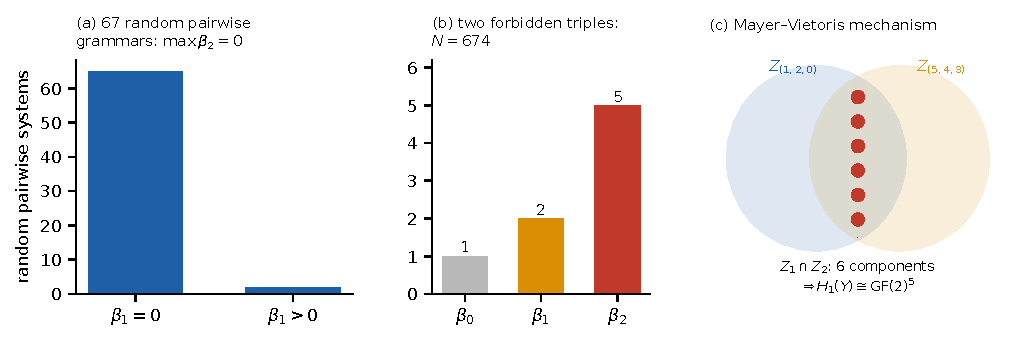
\includegraphics[width=\textwidth]{figures/fig_locality.pdf}
\caption{Pairwise versus triple-local constraints. (a)~$\max\beta_2$ over random pairwise grammars (exact; $\max=0$). (b)~Betti numbers of the system with two forbidden consecutive triples: $(1,2,5)$ with $N=674$ (exact). (c)~The Mayer--Vietoris mechanism: $Z_1\cap Z_2$ has six components, giving $H_1(Y)\cong\F^5$.}\label{fig:locality}
\end{figure}

The intersections $Z_S$ are not acyclic: for $Z_{pqr}$ there are $120$ triples with $Z_{pqr}$ disconnected, which is harmless because only the images of components under $d^1$ matter. The argument uses only the low-degree information (F1)--(F3); a proof by acyclicity of all intersections is not available.
\begin{corollary}[symbolic grammars; analytic]\label[corollary]{cor:symbolic}
For the alphabet $\{S,R,N\}$ with six events of arbitrary categories and arbitrary rule set $G\subseteq\Sigma\times\Sigma$, the admissible set is of the form $A_{G'}$ for a digraph $G'$ on the six events, so \cref{thm:pairwise} applies. All $665$ distinct nonempty proper admissible sets arising from the $28$ category multisets and $512$ rule sets have $\beta_2=0$ and $\beta_3=0$, while $\beta_1$ takes the values $\{0:616,\ 2:42,\ 6:6,\ 8:1\}$ --- positive in $49$ of the $665$. So the pairwise class is restricted in degree $2$ but not in degree $1$.

\end{corollary}
\begin{observation}[symbolic sweeps; bounded]\label[observation]{obs:sym}
(a) Six events with categories $\{S,S,S,R,R,N\}$ and a $9$-bit rule set: all $512$ rule sets give $198$ nonempty and $71$ distinct systems, none with $\beta_2>0$ ($\beta_1>0$ in $9$); the primary target is undefined as a prediction problem (constant). (b) All $28$ size-$6$ category multisets over $\{S,R,N\}$: $783$ distinct systems, $\beta_2=0$ in all, $\beta_1>0$ in $61$. (c) Six distinct symbols with arbitrary transition digraphs, pre-registered: $60{,}000$ draws gave $55{,}296$ distinct systems and none with $\beta_2>0$; a stress sample of $600{,}000$ draws gave $508{,}680$ distinct systems with no $\beta_j>0$ for $j\ge2$ and $11{,}547$ with $\beta_1>0$. The pre-registered transfer predictions were \emph{untestable} (the condition ``$\ge50$ positives'' was not met) and none was falsified. The earlier conjecture that transition-grammar history complexes have no homology above degree $1$ is now a theorem for $\beta_2$ (\cref{thm:pairwise}) and is observed for $\beta_3$.

\end{observation}

\section{Sharpness: constraints on consecutive triples}
\begin{proposition}[triple constraints break the theorem; computer-assisted]\label[proposition]{prop:triple}
Let $A$ be the set of the $674$ orderings of $\{0,\dots,5\}$ containing neither $1,2,0$ nor $5,4,3$ as consecutive entries. Then $(\beta_0,\dots,\beta_5)(K_A)=(1,2,5,0,0,0)$; the $f$-vector is $(674,1606,1240,320,16)$. Mechanism: write $Z_1,Z_2$ for the complexes generated by the flags containing the consecutive triples $(1,2,0)$ and $(5,4,3)$. Computation gives $\Hh_0=\Hh_1=0$ for each, while $Z_1\cap Z_2$ has six components. Reduced Mayer--Vietoris gives
\[
H_1(Y_A)=H_1(Z_1\cup Z_2)\cong\Hh_0(Z_1\cap Z_2)\cong\F^5,
\]
hence $\beta_2(K_A)=5$ by \cref{thm:AD}.

\end{proposition}
\begin{proof}
The Betti numbers are a direct rank computation over $\F$ from the definition. For the mechanism, $Y_A=Z_1\cup Z_2$ and reduced Mayer--Vietoris gives the exact sequence $\Hh_1(Z_1)\oplus\Hh_1(Z_2)\to\Hh_1(Z_1\cup Z_2)\to\Hh_0(Z_1\cap Z_2)\to\Hh_0(Z_1)\oplus\Hh_0(Z_2)$, whose outer terms vanish.
\end{proof}
In an exploratory sample of $19{,}993$ random systems defined by forbidding consecutive triples, $905$ had $\beta_2>0$.

\section{The locality order}
\begin{observation}[locality order]\label[observation]{obs:locality}
For six labels:
\begin{itemize}[nosep]
\item forbidden \emph{adjacencies of order $2$} (consecutive pairs): $\beta_2=0$, proved (\cref{thm:pairwise});
\item forbidden adjacencies of order $3$ (consecutive triples): $\beta_2$ can be positive (\cref{prop:triple});
\item forbidden \emph{prefix sets} (an unbounded-order constraint, since the prefix set is a condition on the whole initial segment): $\beta_2$ can be positive (arithmetic regimes, \cref{ch:topology}); and then $\beta_2=\dim H_1(N[D])$ (\cref{thm:nerve}).
\end{itemize}
The dividing line is how local the forbidden pattern is in the history, not integer divisibility. This is a statement about \emph{six} labels. For the pairwise grammars the cause is concrete: any three adjacency pieces always meet and any two meet in a connected set, so no $1$-cycle can form in $Y_A$.

\end{observation}
The pairwise theorem is not claimed for $k\ne6$: the finite lemmas (F1)--(F3) are specific to $k=6$, and the spectral-sequence argument needs their analogues at the new $k$. We have no purely local criterion for hollowness (\cref{obs:cycle-census}), and no classification of which digraph families give $\beta_1>0$.
